\documentclass[dvipsnames,11pt]{article}
\usepackage{amsmath}

%Hey, if you're using this preamble it means that it was probably written by Stefano Graziosi (me). If you see something that doesn't make sense, feel free to email me at stefano.graziosi@studbocconi.it
%p.s. in case it's not already evident from the preamble, I'm not a professional LaTeX user, so I'm sure there are better ways to do things. I'm just trying to make it work.

%------------------------------------------------------------------------------
%           LAST UPDATE: 30-01-2025
%------------------------------------------------------------------------------

%I don't own copyright on anything, I just literally copied and pasted together a bunch of stuff.

%Credit goes to the original authors.

%------------------------------------------------------------------------------
%           Packages
%------------------------------------------------------------------------------

\usepackage{fancyhdr}
\usepackage[dvipsnames]{xcolor}
\usepackage[many]{tcolorbox}
\usepackage[all]{xy}
\usepackage{tcolorbox}
\usepackage{graphicx}
\usepackage{hyperref}
\usepackage{xcolor}    
\usepackage{wrapfig}
\usepackage{amsmath, amssymb, amsthm}
\usepackage{titlesec}
\usepackage{halloweenmath}
\usepackage{enumitem}
\usepackage{listings}
\usepackage{kantlipsum}
\usepackage{pdfpages}

\usepackage[T1]{fontenc}                            % Font Styling
\usepackage{lmodern,mathrsfs}


\usepackage{mathtools,amsthm,amssymb,amsfonts,bm}   % Math Presets
\usepackage{thmtools,amsmath}
\usepackage{array,tabularx,booktabs}                % Table Presets
\usepackage{graphicx,wrapfig,float,caption}         % Figure Presets
\usepackage{setspace,multicol}                      % Text Presets
\usepackage{tikz,physics}                           % Physics Presets

\usepackage{titlepic}
\usepackage{pdfpages}

%------------------------------------------------------------------------------
%           Geometry
%------------------------------------------------------------------------------

\usepackage[a4paper,margin=1in]{geometry}
%\usepackage[margin=1in]{geometry}

%------------------------------------------------------------------------------
%           Chapter and section formatting
%------------------------------------------------------------------------------

%\renewcommand{\chaptername}{Lecture}
%\renewcommand\thesection{P~\arabic{section}}

\renewcommand{\thefigure}{\thesection-\arabic{figure}}
\renewcommand{\thetable}{\thesection-\arabic{table}}

%------------------------------------------------------------------------------
%           Colours
%------------------------------------------------------------------------------

\definecolor{sgblue}{rgb}{0, 169, 211}
\definecolor{sggreen}{rgb}{0, 164, 0}
\definecolor{sgpurple}{rgb}{99, 0, 165}
\definecolor{sgyellow}{rgb}{255, 211, 0}
\definecolor{sgorange}{rgb}{255, 127, 20}

\definecolor{sbblue}{rgb}{219, 248, 254}
\definecolor{sbgreen}{rgb}{223, 255, 218}
\definecolor{sbpurple}{rgb}{241, 220, 255}

\definecolor{codegreen}{rgb}{0,0.6,0}
\definecolor{codegray}{rgb}{0.5,0.5,0.5}
\definecolor{codepurple}{rgb}{0.58,0,0.82}
\definecolor{backcolour}{rgb}{0.95,0.95,0.92}

%------------------------------------------------------------------------------
%           Environments
%------------------------------------------------------------------------------

%Standard \latex box

\newtcolorbox{mybox}[3][]
{
  colframe = #2!25,
  colback  = #2!10,
  coltitle = #2!20!black,  
  title    = {#3},
  #1,
}

%Standard "Problem" environment

\newtheorem{problem}{Problem}

%Personalised "Solution" environment

\newenvironment{solution}[1][\it{\textcolor{MidnightBlue}{Solution}}]{\textbf{#1. } }{\textcolor{MidnightBlue}{$\square$}}


% ----------------------------------------------------------------------
%           Special Environments 
% ----------------------------------------------------------------------

\newlength{\spacelength}
\settowidth{\spacelength}{\normalfont\ }
\declaretheoremstyle[
    headfont={\bfseries\sffamily\footnotesize},
    notefont={\normalfont},
    bodyfont={\normalfont},
    headpunct={\relax},%\newline,
    headformat={%
        \makebox[0pt][r]{\NAME\ \NUMBER\hspace{\marginparsep}}\hskip-\spacelength{\normalsize\NOTE}},
]{theorem}

\tcolorboxenvironment{theorem}{
  boxrule=0pt,
  boxsep=0pt,
  colback={White},
  enhanced jigsaw, 
  borderline west={1pt}{0pt}{ForestGreen},
  sharp corners,
  before skip=10pt,
  after skip=10pt,
  left=5pt,
  right=5pt,
  breakable,
}

\declaretheorem[style=theorem]{proposition}

\let\proof\relax
\let\endproof\relax

\declaretheoremstyle[
    headfont={\bfseries\sffamily\footnotesize},
    notefont={\normalfont},
    bodyfont={\normalfont},
    headpunct={\relax},%\newline,
    headformat={%
        \makebox[0pt][r]{\NAME\ \NUMBER\hspace{\marginparsep}}\hskip-\spacelength{\normalsize\NOTE}},
]{theorem}

\tcolorboxenvironment{proposition}{
  boxrule=0pt,
  boxsep=0pt,
  colback={White},
  enhanced jigsaw, 
  borderline west={1pt}{0pt}{Mulberry},
  sharp corners,
  before skip=10pt,
  after skip=10pt,
  left=5pt,
  right=5pt,
  breakable,
}

\declaretheorem[style=theorem]{theorem}

\let\proof\relax
\let\endproof\relax

\declaretheoremstyle[
    headfont={\small\scshape},
    notefont={\normalfont},
    bodyfont={\normalfont},
    headpunct={\relax},
    headformat={%
        \makebox[0pt][r]{\NAME\hspace{\marginparsep}}\hskip-\spacelength{\NOTE}},
]{proof}

\tcolorboxenvironment{proof}{
  boxrule=0pt,
  boxsep=0pt,
  blanker,
  borderline west={1pt}{0pt}{black},
  before skip=10pt,
  after skip=10pt,
  left=5pt,
  right=5pt,
  breakable,
}

\declaretheoremstyle[
    headfont={\footnotesize\itshape},
    notefont={\normalfont},
    bodyfont={\normalfont},
    headpunct={\relax},
    headformat={%
        \makebox[0pt][r]{\NAME\hspace{\marginparsep}}\hskip-\spacelength{\NOTE}},
]{claim}

\declaretheorem[
    style=proof,
    qed=\qedsymbol]{proof}

\declaretheorem[style=claim]{Intuition}

\theoremstyle{theorem}
\newtheorem{ques}{Question}

\theoremstyle{theorem}
\newtheorem{definition}{Definition}
\tcolorboxenvironment{definition}{
  boxrule=0pt,
  boxsep=0pt,
  colback={White},
  enhanced jigsaw, 
  borderline west={1pt}{0pt}{Cerulean},
  sharp corners,
  before skip=10pt,
  after skip=10pt,
  left=5pt,
  right=5pt,
  breakable,
}

\theoremstyle{theorem}
\newtheorem{lemma}{Lemma}
\tcolorboxenvironment{lemma}{
  boxrule=0pt,
  boxsep=0pt,
  blanker,
  borderline west={1pt}{0pt}{Rhodamine},
  before skip=10pt,
  after skip=10pt,
  sharp corners,
  left=5pt,
  right=5pt,
  breakable,
}

\theoremstyle{theorem}
\newtheorem{remark}{Remark}
\tcolorboxenvironment{remark}{
  boxrule=0pt,
  boxsep=0pt,
  colback={White},
  enhanced jigsaw, 
  borderline west={1pt}{0pt}{BurntOrange},
  before skip=10pt,
  after skip=10pt,
  sharp corners,
  left=5pt,
  right=5pt,
  breakable,
}

\theoremstyle{theorem}
\newtheorem{corollary}{Corollary}
\tcolorboxenvironment{corollary}{
  boxrule=0pt,
  boxsep=0pt,
%  colback={White!100!WildStrawberry},
  enhanced jigsaw,
  borderline west={1pt}{0pt}{WildStrawberry},
  before skip=10pt,
  after skip=10pt,
  sharp corners,
  left=5pt,
  right=5pt,
  breakable,
}

\theoremstyle{theorem}
\newtheorem{example}{Example}
\tcolorboxenvironment{example}{
  boxrule=0pt,
  boxsep=0pt,
  blanker,
  borderline west={1pt}{0pt}{Dandelion},
  before skip=10pt,
  after skip=10pt,
  sharp corners,
  left=5pt,
  right=5pt,
  breakable,
}


\theoremstyle{claim}
\newtheorem{intu}{Intuition}

\theoremstyle{claim}
\newtheorem{solu}{Solution}

%------------------------------------------------------------------------------
%           Code Listing Environment
%------------------------------------------------------------------------------

\lstdefinestyle{mystyle}{
    backgroundcolor=\color{backcolour},   
    commentstyle=\color{codegreen},
    keywordstyle=\color{magenta},
    numberstyle=\tiny\color{codegray},
    stringstyle=\color{codepurple},
    basicstyle=\ttfamily\footnotesize,
    breakatwhitespace=false,         
    breaklines=true,                 
    captionpos=b,                    
    keepspaces=true,                 
    numbers=left,                    
    numbersep=5pt,                  
    showspaces=false,                
    showstringspaces=false,
    showtabs=false,                  
    tabsize=2
}

\lstset{style=mystyle}

\setlength{\headheight}{25pt} % Non so perché ma senza questo da un piccolo errore

\pagestyle{fancy}
\fancyhf{} 
\fancyhead[L]{\textsc{\footnotesize{PhD in Economics and Finance} \\ \small{40313 Introd. to Probability}}} 
\fancyhead[R]{\textsc{\small Graziosi \\ Natalucci}} 
\fancyhead[C]{\textbf{Problem set 1}}
\fancyfoot[C]{\thepage} 
\renewcommand{\headrulewidth}{0.4pt} 
\renewcommand{\footrulewidth}{0pt}

\begin{document}

\section*{Question 1}

\textbf{1.} A coin is tossed infinitely many times. For every $n=2,3,4,...$ , let $A_n$ be the event “a block of
heads of length n starting from toss n ” (that is heads at tosses $n,\dots,2n-1$, tails at tosses $n-1$ and $2n$).\\

    \begin{enumerate}[label=\alph*.]
        \item Find the probability of $A_n$
    
            \begin{solution}
    
                Let $H_i$ (resp. $T_i$) denote “head (resp. tail) at toss $i$.” Then
                \[
                A_n \;=\; T_{n-1}\;\cap\;\Big(\bigcap_{i=n}^{2n-1} H_i\Big)\;\cap\;T_{2n}.
                \]
                By independence of coin tosses, 
                \[
                \mathbb P(A_n)=\mathbb P(T_{n-1})\cdot\prod_{i=n}^{2n-1}\mathbb P(H_i)\cdot \mathbb P(T_{2n}) = \Big(\tfrac12\Big)\cdot\Big(\tfrac12\Big)^{n}\cdot\Big(\tfrac12\Big)=2^{-(n+2)}.
                \]
                
            \end{solution}
            
        \item Is $A_n$ an increasing sequence?
    
            \begin{solution}
    
                \textbf{No}. For an increasing sequence we would need $A_n\subseteq A_{n+1}$ for all $n$. But $A_n$ requires $T_{2n}$ while $A_{n+1}$ requires $H_{2n}$, so $A_n\cap A_{n+1}=\varnothing$. Hence $A_n\not\subseteq A_{n+1}$.
                
            \end{solution}
            
        \item Is $A_n$ a decreasing sequence?
    
            \begin{solution}
    
                \textbf{No}. A decreasing sequence would satisfy $A_{n+1}\subseteq A_n$ for all $n$, which again fails since $A_n\cap A_{n+1}=\varnothing$ and both events are nonempty.
                
            \end{solution}
            
        \item Is $A_n$ a convergent sequence?
    
            \begin{solution}
    
                Recall that $\liminf_n A_n=\bigcup_{m}\bigcap_{n\ge m}A_n$ (“$A_n$ ultimately”) and  $\limsup_n A_n=\bigcap_{m}\bigcup_{n\ge m}A_n$ (“$A_n$ infinitely often”). Because $A_n\cap A_{n+1}=\varnothing$, it is impossible that $A_n$ occurs for all sufficiently large $n$, so $\liminf_n A_n=\varnothing$. 
                
                On the other hand, one can construct sequences where $A_n$ occurs for infinitely many $n$ (e.g. arrange disjoint blocks $TH^nT$ spaced far apart), so $\limsup_n A_n\neq\varnothing$. 
                
                Thus $\liminf_n A_n\ne\limsup_n A_n$ and $(A_n)$ does not converge.
                
            \end{solution}
            
        \item What is the probability that $A_n$ occurs infinitely often?
    
            \begin{solution}

                We have 
                \[
                \sum_{n=2}^\infty \mathbb P(A_n)=\sum_{n=2}^\infty 2^{-(n+2)}=\tfrac18<\infty.
                \]
                By the First Borel–Cantelli lemma, $\mathbb P(A_n\ \text{i.o.})=0$.
                
            \end{solution}
            
        \item What is the probability that $A_n$ occurs ultimately?
    
            \begin{solution}
    
                Since $\mathbb P(A_n)=2^{-(n+2)}\to 0$ and $\mathbb P(\liminf_n A_n)\le \liminf_{n\to\infty}\mathbb P(A_n)$, we get 
                \[ \mathbb P(A_n\ \text{ultimately})=\mathbb P(\liminf_n A_n)=0.
                \] 
                
                (Equivalently, $\liminf_n A_n\subseteq \limsup_n A_n$ and part (e) already gave $\mathbb P(\limsup_n A_n)=0$.)
                
            \end{solution}
            
    \end{enumerate}

%%%%%%%%%%%%%%%%%%%%%%%%%%%%%%%%%%%%%%%%%%%%

\section*{Question 2}

\textbf{2.} Simulate in Matlab or in Python 1000 tossing of a fair coin.

    \begin{enumerate}
        \item Count the number of heads and the number of tails.

            \begin{solution}

\begin{lstlisting}[language=python]
import numpy as np

rng = np.random.default_rng(40313)  # fixed seed for reproducibility
n = 1000

# True = Head, False = Tail
tosses = rng.random(n) < 0.5

heads = int(tosses.sum())
tails = n - heads

print(f"Heads: {heads}, Tails: {tails}")
\end{lstlisting}

                Heads: 477, Tails: 523
            
            \end{solution}
        
        \item Find the frequency of heads as a function of $n$ ($n=1,\dots,1000$) and represent the function.

            \begin{solution}
    
\begin{lstlisting}[language=python]
import numpy as np
import matplotlib.pyplot as plt

rng = np.random.default_rng(2024)
n = 1000

# 1 = Head, 0 = Tail
tosses = (rng.random(n) < 0.5).astype(int)

cum_heads = np.cumsum(tosses)
n_vals = np.arange(1, n + 1)
freq = cum_heads / n_vals

plt.figure()
plt.plot(n_vals, freq, label="Observed head frequency")
plt.axhline(0.5, linestyle="--", linewidth=1, label="Theoretical p=0.5")
plt.xlabel("n (number of tosses)")
plt.ylabel("Frequency of heads up to n")
plt.title("Cumulative frequency of heads (fair coin)")
plt.legend()
plt.show()
\end{lstlisting}

                \begin{figure}[ht]
                    \centering
                    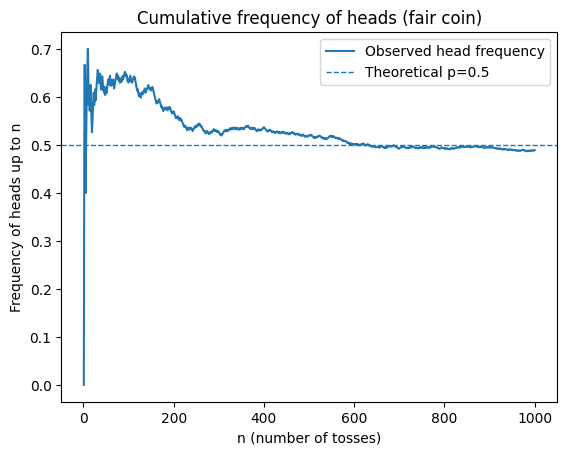
\includegraphics[width=0.5\linewidth]{Q2b.png}
                    \caption{Cumulative Frequency of Heads (Fair Coin)}
                    \label{fig:Q2b}
                \end{figure}
                
            \end{solution}
            
        \item Count the number of blocks of heads of length 2 (that is sequences (THHT)).

            \begin{solution}
    
\begin{lstlisting}[language=python]
import numpy as np

def count_THHT(tosses):
    """
    Count occurrences of the pattern Tail-Head-Head-Tail (THHT).
    Accepts either:
      - a string like "THHTHT...", or
      - an iterable of "H"/"T" characters.
    """
    s = tosses if isinstance(tosses, str) else "".join(tosses)
    return sum(1 for i in range(len(s) - 3) if s[i:i+4] == "THHT")

rng = np.random.default_rng(40313) # fixed seed for reproducibility
n = 1000

tosses = np.where(rng.random(n) < 0.5, "H", "T")  # array of "H"/"T"

print("THHT count:", count_THHT(tosses))
\end{lstlisting}

                THHT count: 60
                
            \end{solution}
            
        \item Repeat the above calculations for a coin with probability of heads=3/4.

            \begin{solution}
    
\begin{lstlisting}[language=python]
import numpy as np
import matplotlib.pyplot as plt

# --- Setup ---
rng = np.random.default_rng(2024)
n = 1000
p = 0.75  # probability of Heads

# Simulate: 1 = Head, 0 = Tail
tosses = (rng.random(n) < p).astype(int)

# (a) Counts
heads = int(tosses.sum())
tails = n - heads
print(f"Heads: {heads}, Tails: {tails}")

# (b) Frequency of heads vs n
cum_heads = np.cumsum(tosses)
n_vals = np.arange(1, n + 1)
freq = cum_heads / n_vals

plt.figure()
plt.plot(n_vals, freq, label="Observed head frequency")
plt.axhline(p, linestyle="--", linewidth=1, label=f"Theoretical p={p}")
plt.xlabel("n (number of tosses)")
plt.ylabel("Frequency of heads up to n")
plt.title("Cumulative frequency of heads (biased coin, p=0.75)")
plt.legend()
plt.show()

# (c) Count occurrences of the pattern THHT
def count_THHT(tosses_ht_or_str):
    """
    Count occurrences of Tail-Head-Head-Tail (THHT).
    Accepts a string of 'H'/'T' or an iterable of 'H'/'T'.
    """
    s = tosses_ht_or_str if isinstance(tosses_ht_or_str, str) else "".join(tosses_ht_or_str)
    return sum(1 for i in range(len(s) - 3) if s[i:i+4] == "THHT")

# Convert to 'H'/'T' and count
ht = np.where(tosses == 1, "H", "T")
thht_count = count_THHT(ht)
print(f"Occurrences of 'THHT': {thht_count}")
\end{lstlisting}

                Heads: 740, Tails: 260

                    \begin{figure}[ht]
                        \centering
                        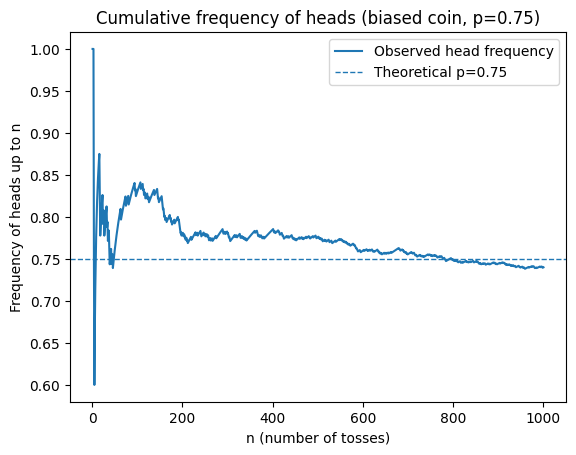
\includegraphics[width=0.5\linewidth]{Q2d.png}
                        \caption{Cumulative Frequency of Heads (Biased Coin)}
                        \label{fig:placeholder}
                    \end{figure}

                Occurrences of 'THHT': 46
                
            \end{solution}
            
    \end{enumerate}

\end{document}
